\subsection{Метод с использование неявной схемы}
Используемая консервативная разностная схема для исходного уравнения (\ref{MainNoDim}) для неравномерных сеток в поперечном сечении была предложена в (\cite{SweepScheme}). Она выглядит следующим образом:

\begin{equation}\label{sweep_diff_sys}
    \left\{
    \begin{aligned}
        2i\frac{h_1}{2}\frac{\hat{E}_{0,j}-E^k_{0,j}}{\Delta z} &= \frac{1}{2}\left(\frac{\hat{E}_{1,j}-\hat{E}_{0,j}}{h_1}\right) + \frac{1}{2}\left(\frac{E^k_{1,j}-E^k_{0,j}}{h_0}\right)\\
        2i\frac{h_{i+1}+h_i}{2}\frac{\hat{E}_{i,j}-E^k_{i,j}}{\Delta z} &= \frac{1}{2}\left(\frac{\hat{E}_{i+1,j}}{h_{i+1}} -\left(\frac{1}{h_{i+1}} + \frac{1}{h_i}\right)\hat{E}_{i,j} + \frac{\hat{E}_{i-1,j}}{h_i}\right) \\
        &\qquad+ \frac{1}{2}\left(\frac{E^k_{i+1,j}}{h_{i+1}} -\left(\frac{1}{h_{i+1}} + \frac{1}{h_i}\right)E^k_{i,j} + \frac{E^k_{i-1,j}}{h_i}\right),\quad i=1,\ldots N\\
        2i\frac{h_N}{2}\frac{\hat{E}_{N,j}-E^k_{N,j}}{\Delta z} &= \frac{1}{2}\left(\frac{\hat{E}_{N,j}-\hat{E}_{N-1,j}}{h_N}\right) + \frac{1}{2}\left(\frac{E^k_{N,j}-E^k_{N,j}}{h_{N-1}}\right)
    \end{aligned}
    \right.
\end{equation}

Указанная схема осуществляет расчет <<дифракции по $x$>>.
Аналогичная система разностных уравнений рассчитывает <<дифракцию по $y$>>.
Если шаг сетки равномерный, то есть $h_i=x_i-x_{i-1}=const$, то схема переходит в хорошо известную схему Кранка-Николсона.
Учет керровской нелинейности осуществляется в рамках описан в разделе \ref{SplitMethod}.

Указанная система является системой относительно значений поля на промежуточном слое $\hat{E}_{i,j}$.
Матрица системы трехдиагональна и решается методом прогонки (ссылка на Калиткина).
Рассмотрим вариант параллельной реализации прогонки.

\begin{figure}[h]
    \begin{center}
        \begin{minipage}{0.48\linewidth}
            \center{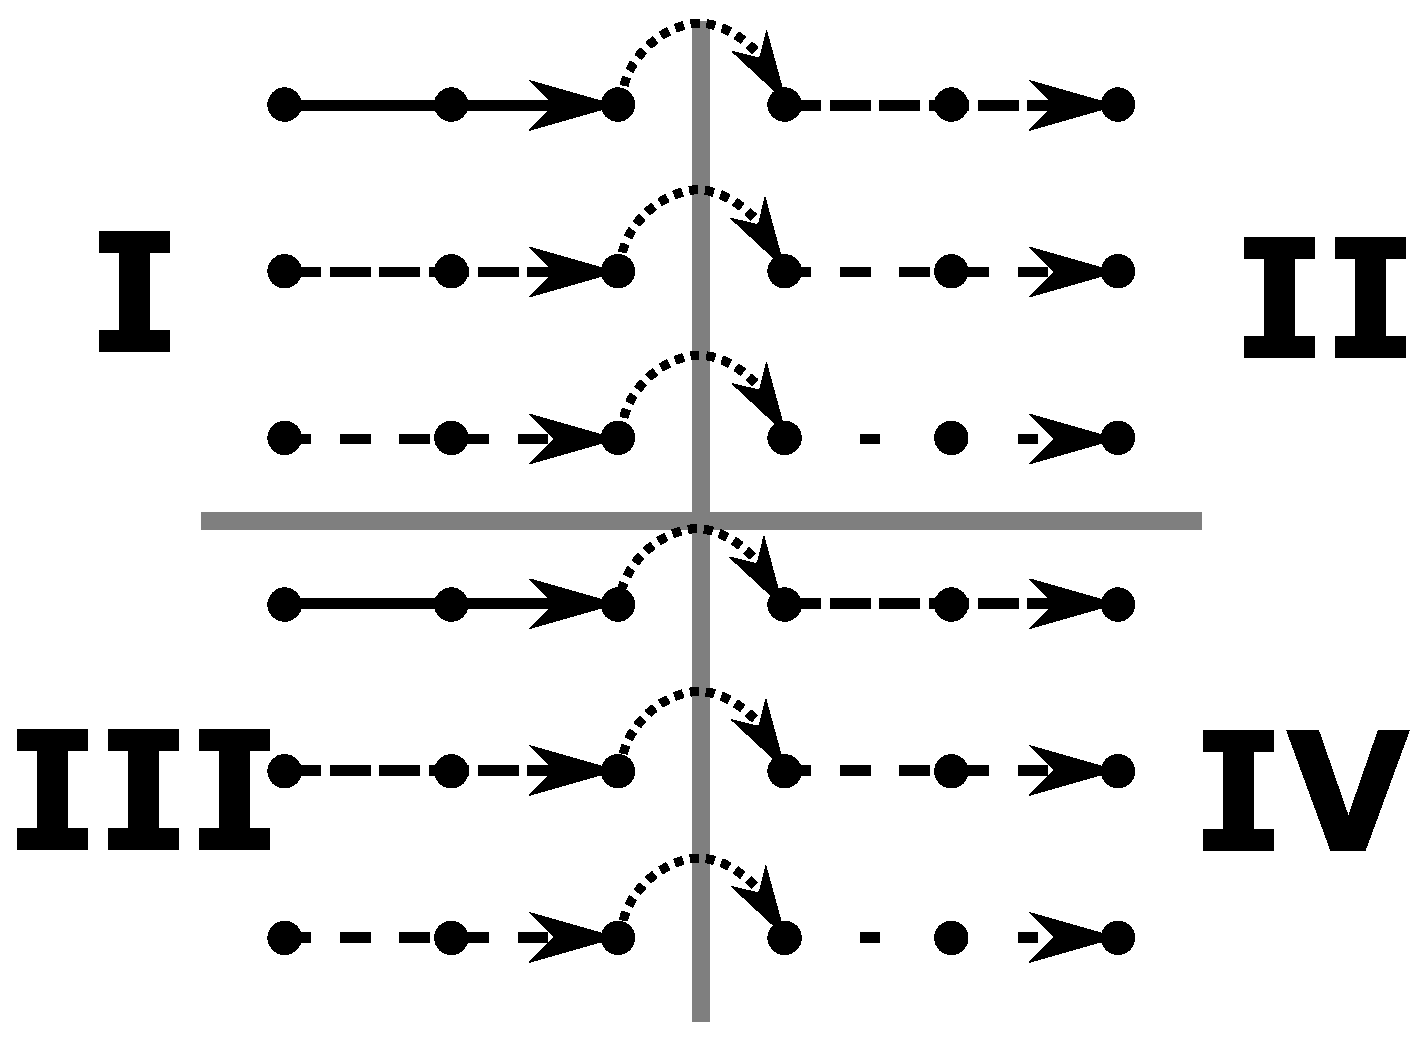
\includegraphics[width=0.95\linewidth]{\imagesdir/sweep_method_forward.eps}} \\
            \caption{Метод с использованием неявной схемы. Прямая прогонка.}
            \label{img:sweepforward}
        \end{minipage}
        \hfill
        \begin{minipage}{0.48\linewidth}
            \center{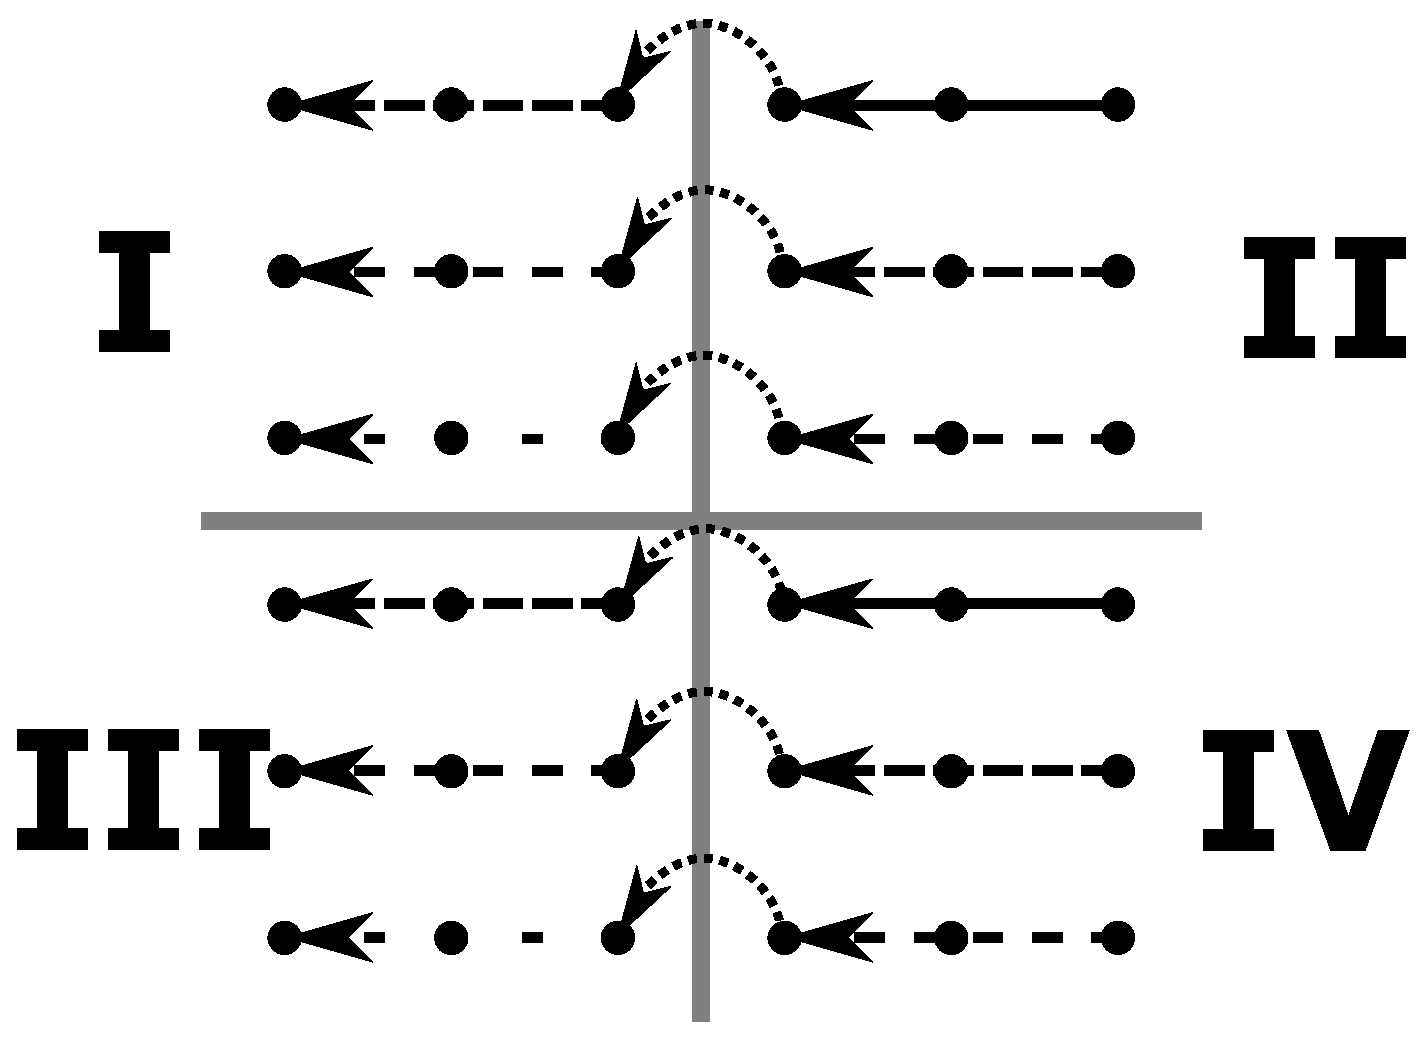
\includegraphics[width=0.95\linewidth]{\imagesdir/sweep_method_backward.eps}} \\
            \caption{Метод с использованием неявной схемы. Обратная прогонка.}
            \label{img:sweepbackward}
        \end{minipage}
    \end{center}
\end{figure}

На рис. \ref{img:sweepforward}, \ref{img:sweepbackward} черными точками изображены точки расчетной сетки.
Вертикальная и горизонтальная светло-серые прямые показывают разбиение матрицы поперечного сечения между процессами.
Римские цифры обозначают номера процессов.
Цветные стрелки соответствуют вычислению прогоночных коэффициентов.
Серые стрелки отображают обмены данными между процессами.

Первому расчетному шагу соответствуют стрелки красного цвета.
Для цикла прямой прогонки их выполняют процессы первого столбца матрицы процессов.
Далее эти процессы пересылают посчитанные коэффициенты в граничной точке соседнему справа процессу.
Следующий такт отображен стрелками зеленого цвета, далее следуют синие и коричневые стрелки.
Таким образом, по каждой строке матрицы процессов запускается конвейерная схема параллельных вычислений.

В цикле обратной прогонки конвейерная схема запускается в обратную сторону (соответствие цвета стрелок и порядка выполнения расчетных операций то же).
Пересылке теперь подвергаются расчитанные значения поля.

Отметим две особенности метода.
Во-первых, поскольку цикл обратной прогонки запускается после окончания прямой прогонки по всем строкам расчетной сетки, то необходимо хранить в памяти прогоночные коэффициенты для всех строк, то есть необходима дополнительная матрица для прогоночных коэффициентов того же размера, что и матрица поля.
Во-вторых, для расчета коэффициентов, фигурирующих в разностной системе (\ref{sweep_diff_sys}), необходим обмен значениями поля в граничных областях.

Отметим также, что для высокой эффективности параллельного алгоритма необходимо, чтобы количество строк матрицы поля у отдельного процесса было существенно больше количества процессов в строке матрицы процессов.
Действительно, если число строк у отдельного процесса равно $N_{loc}$, а число процессов в строке матрицы процессов равно $q$ (на рис. \ref{img:sweepforward}, \ref{img:sweepbackward} $N_{loc}=3$, $q=2$), то на цикл прямой прогонки потребуется $N_{loc}+q$ итераций.
Таким образом, верхняя оценка на эффективность имеет вид:
\begin{equation}
    E_n\leqslant\frac{N_{loc}q^2}{q^2(N_{loc} + q)}=\frac{1}{1+q/N_{loc}}.
\end{equation}

В этом соотношении не учтены потери времени на пересылки и синхронизацию процессов. 